\chapter{REGALE}\label{chap:4_REGALE}
%COSA
REGALE\cite{REGALE} è un progetto finanziato dall'UE\cite{ue_REGALE} nato ad Aprile 2021 che opera nell'ambito del Power Management in sistemi ad High-Performance Computing ed in particolare si è focalizzato su sistemi Exascale\footnote{Exascale: capace di eseguire operazioni nell'ordine di ExaFlops ($10^{18}$)}.

\section{Obbiettivi}
Il loro principale obbiettivo è quello di aprire la strada alla prossima generazione di applicazioni per HPC, riunendo accademici e centri europei di supercalcolo. Il progetto si pone di definire un'architettura open-source con l'intenzione di costruire un prototipo in grado di dotare i sistemi di HPC dei meccanismi e delle politiche necessari per garantire un utilizzo delle risorse efficace\cite{ue_REGALE}. Per farlo sono inoltre state definite delle politiche da seguire durante lo sviluppo di tutto il progetto:
\begin{itemize}
    \item Effettivo utilizzo delle risorse disponibili, tramite aumento del throughput del sistema e la minimizzazione della \emph{Performance Degradation} sotto vincoli di potenza;
    \item Ampia applicabilità attraverso l'inseguimento di concetti come scalabilità, indipendenza dalle piattaforme ed estensibilità;
    \item Facilità di implementazione tramite la creazione di una infrastruttura flessibile, e che gestisca in automatico le risorse.
\end{itemize}


\section{Power Stack}
L'intero progetto di Power Stack, durante il suo sviluppo, si è basato su strumenti come MPI library\cite{mpi}, SLURM\cite{slurm}, o DCDB\cite{dcdb}. Inoltre, è stato deciso di introdurre software open-source che potessero soddisfare le esigenze del modello di Power Stack~\ref{fig:powerstackscheme}. Infatti sono stati valutati e selezionati diversi applicativi (molti dei quali prodotti dai partner, come mostrati in tabella~\ref{table:REGALE}) anche con ruoli analoghi, per soddisfare diverse esigenze.
\begin{table}[ht]
    \centering
    \begin{tabular}{l|l|l}
    \hline
    \textbf{Tool} & \textbf{Partner} & \textbf{Ruolo all'interno di REGALE} \\
    \hline
    SLURM & TUM & System Manager \\
    \hline
    OAR & UGA & System Manager \\
    \hline
    DCDB & LRZ & Monitor, Monitoring Data \\
    \hline
    BEO & ATOS & Monitor, Node Manager, Monitoring Data \\
    \hline
    BDBO & ATOS & Monitor, Job Manager \\
    \hline
    EAR & BSC & Monitor, Node Manager, Job Manager, Monitoring Data \\
    \hline
    Melissa & UGA & Workflow Engine \\
    \hline
    RYAX & RYAX & Workflow Engine \\
    \hline
    Examon & E4/UNIBO & Monitor, Monitoring Data \\
    \hline
    COUNTDOWN & CINECA/UNIBO & Job Manager \\
    \hline
    PULPcontroller & UNIBO & Node Manager \\
    \hline
    BeBiDa & RYAX & System Manager \\
    \hline
\end{tabular}
\caption{Software introdotti all'interno di REGALE con il partner che li ha prodotti e il loro ruolo}\label{table:REGALE}
\end{table}

\begin{figure}[H]
    \centering
    \begin{subfigure}[b]{0.50\textwidth}
    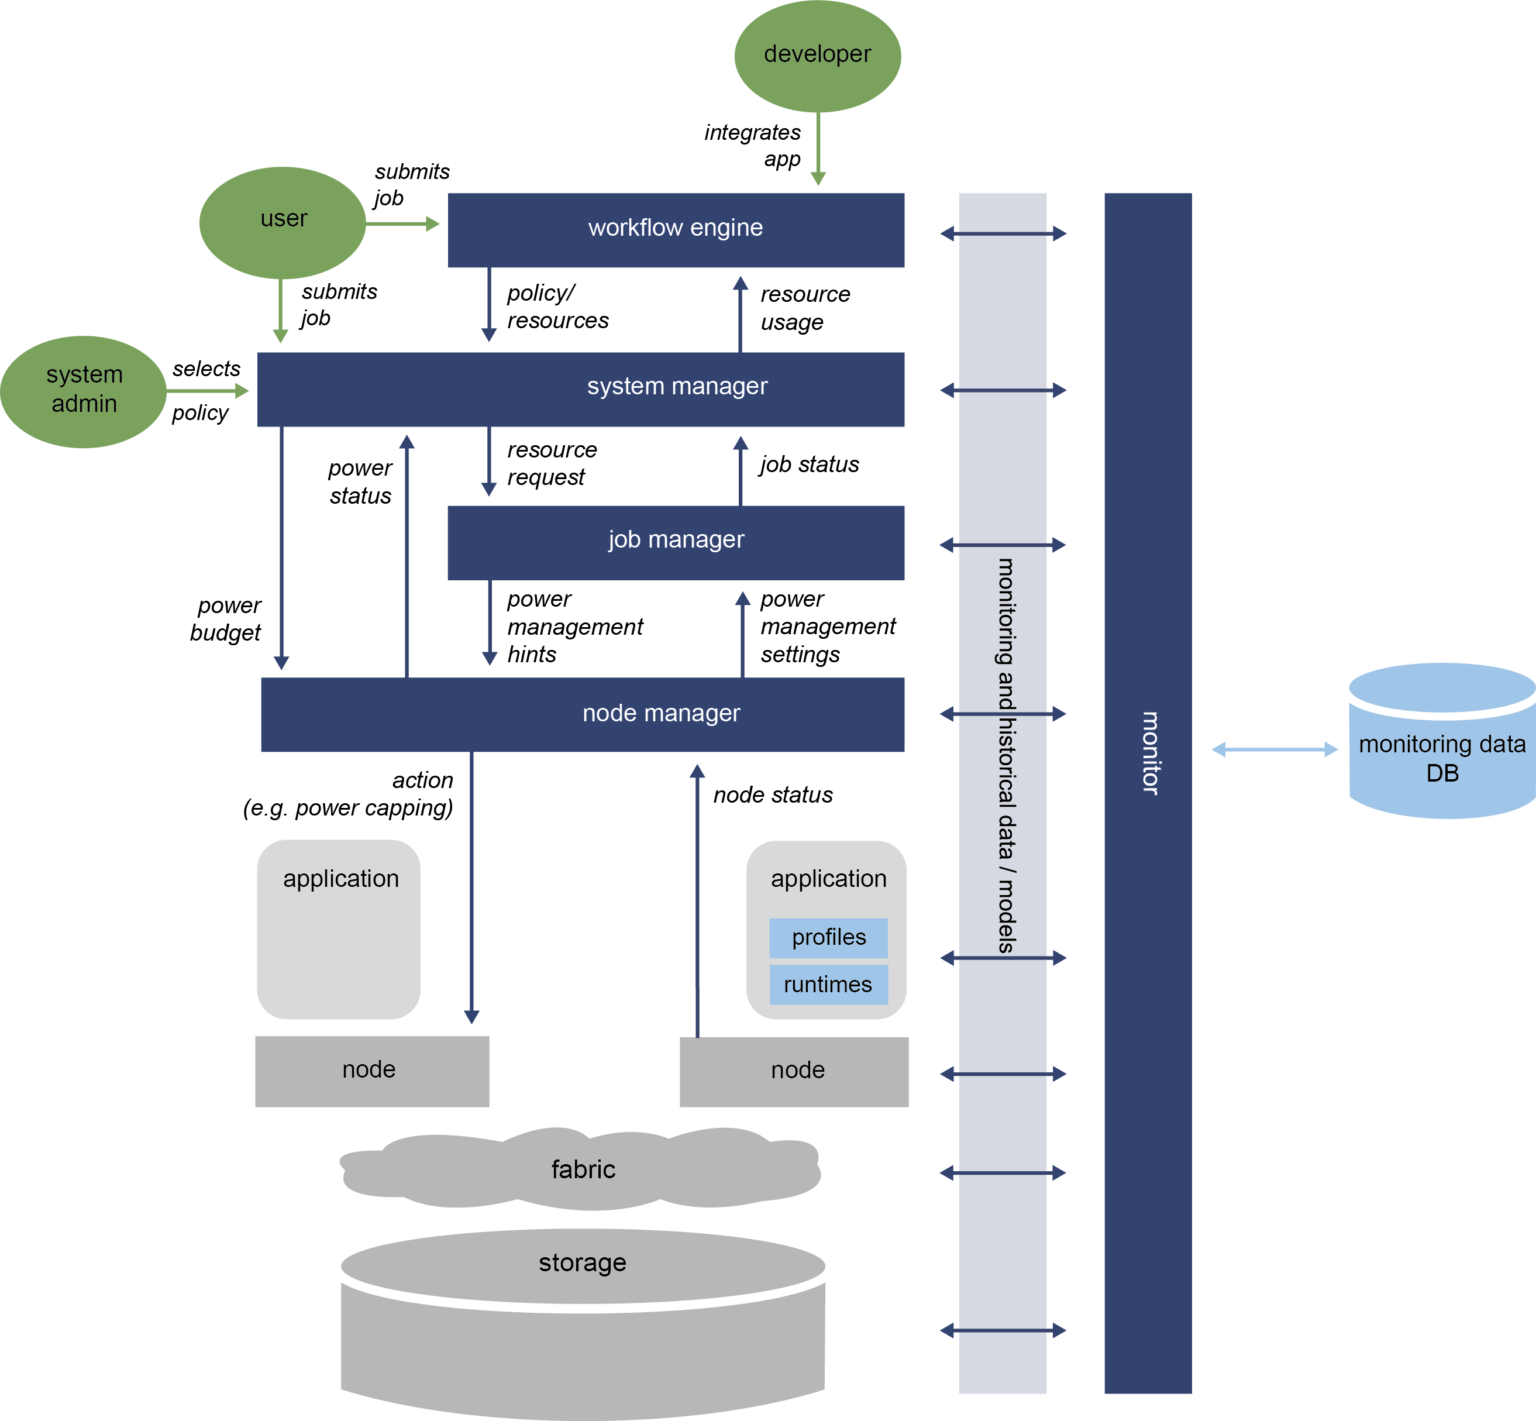
\includegraphics[width=\textwidth]{img/REGALE-Architecture-1536x1421.png}
    \caption{Modello di Power Stack Regale}\label{fig:powerstackscheme}
    \end{subfigure}
    \hfill
    \begin{subfigure}[b]{0.50\textwidth}
    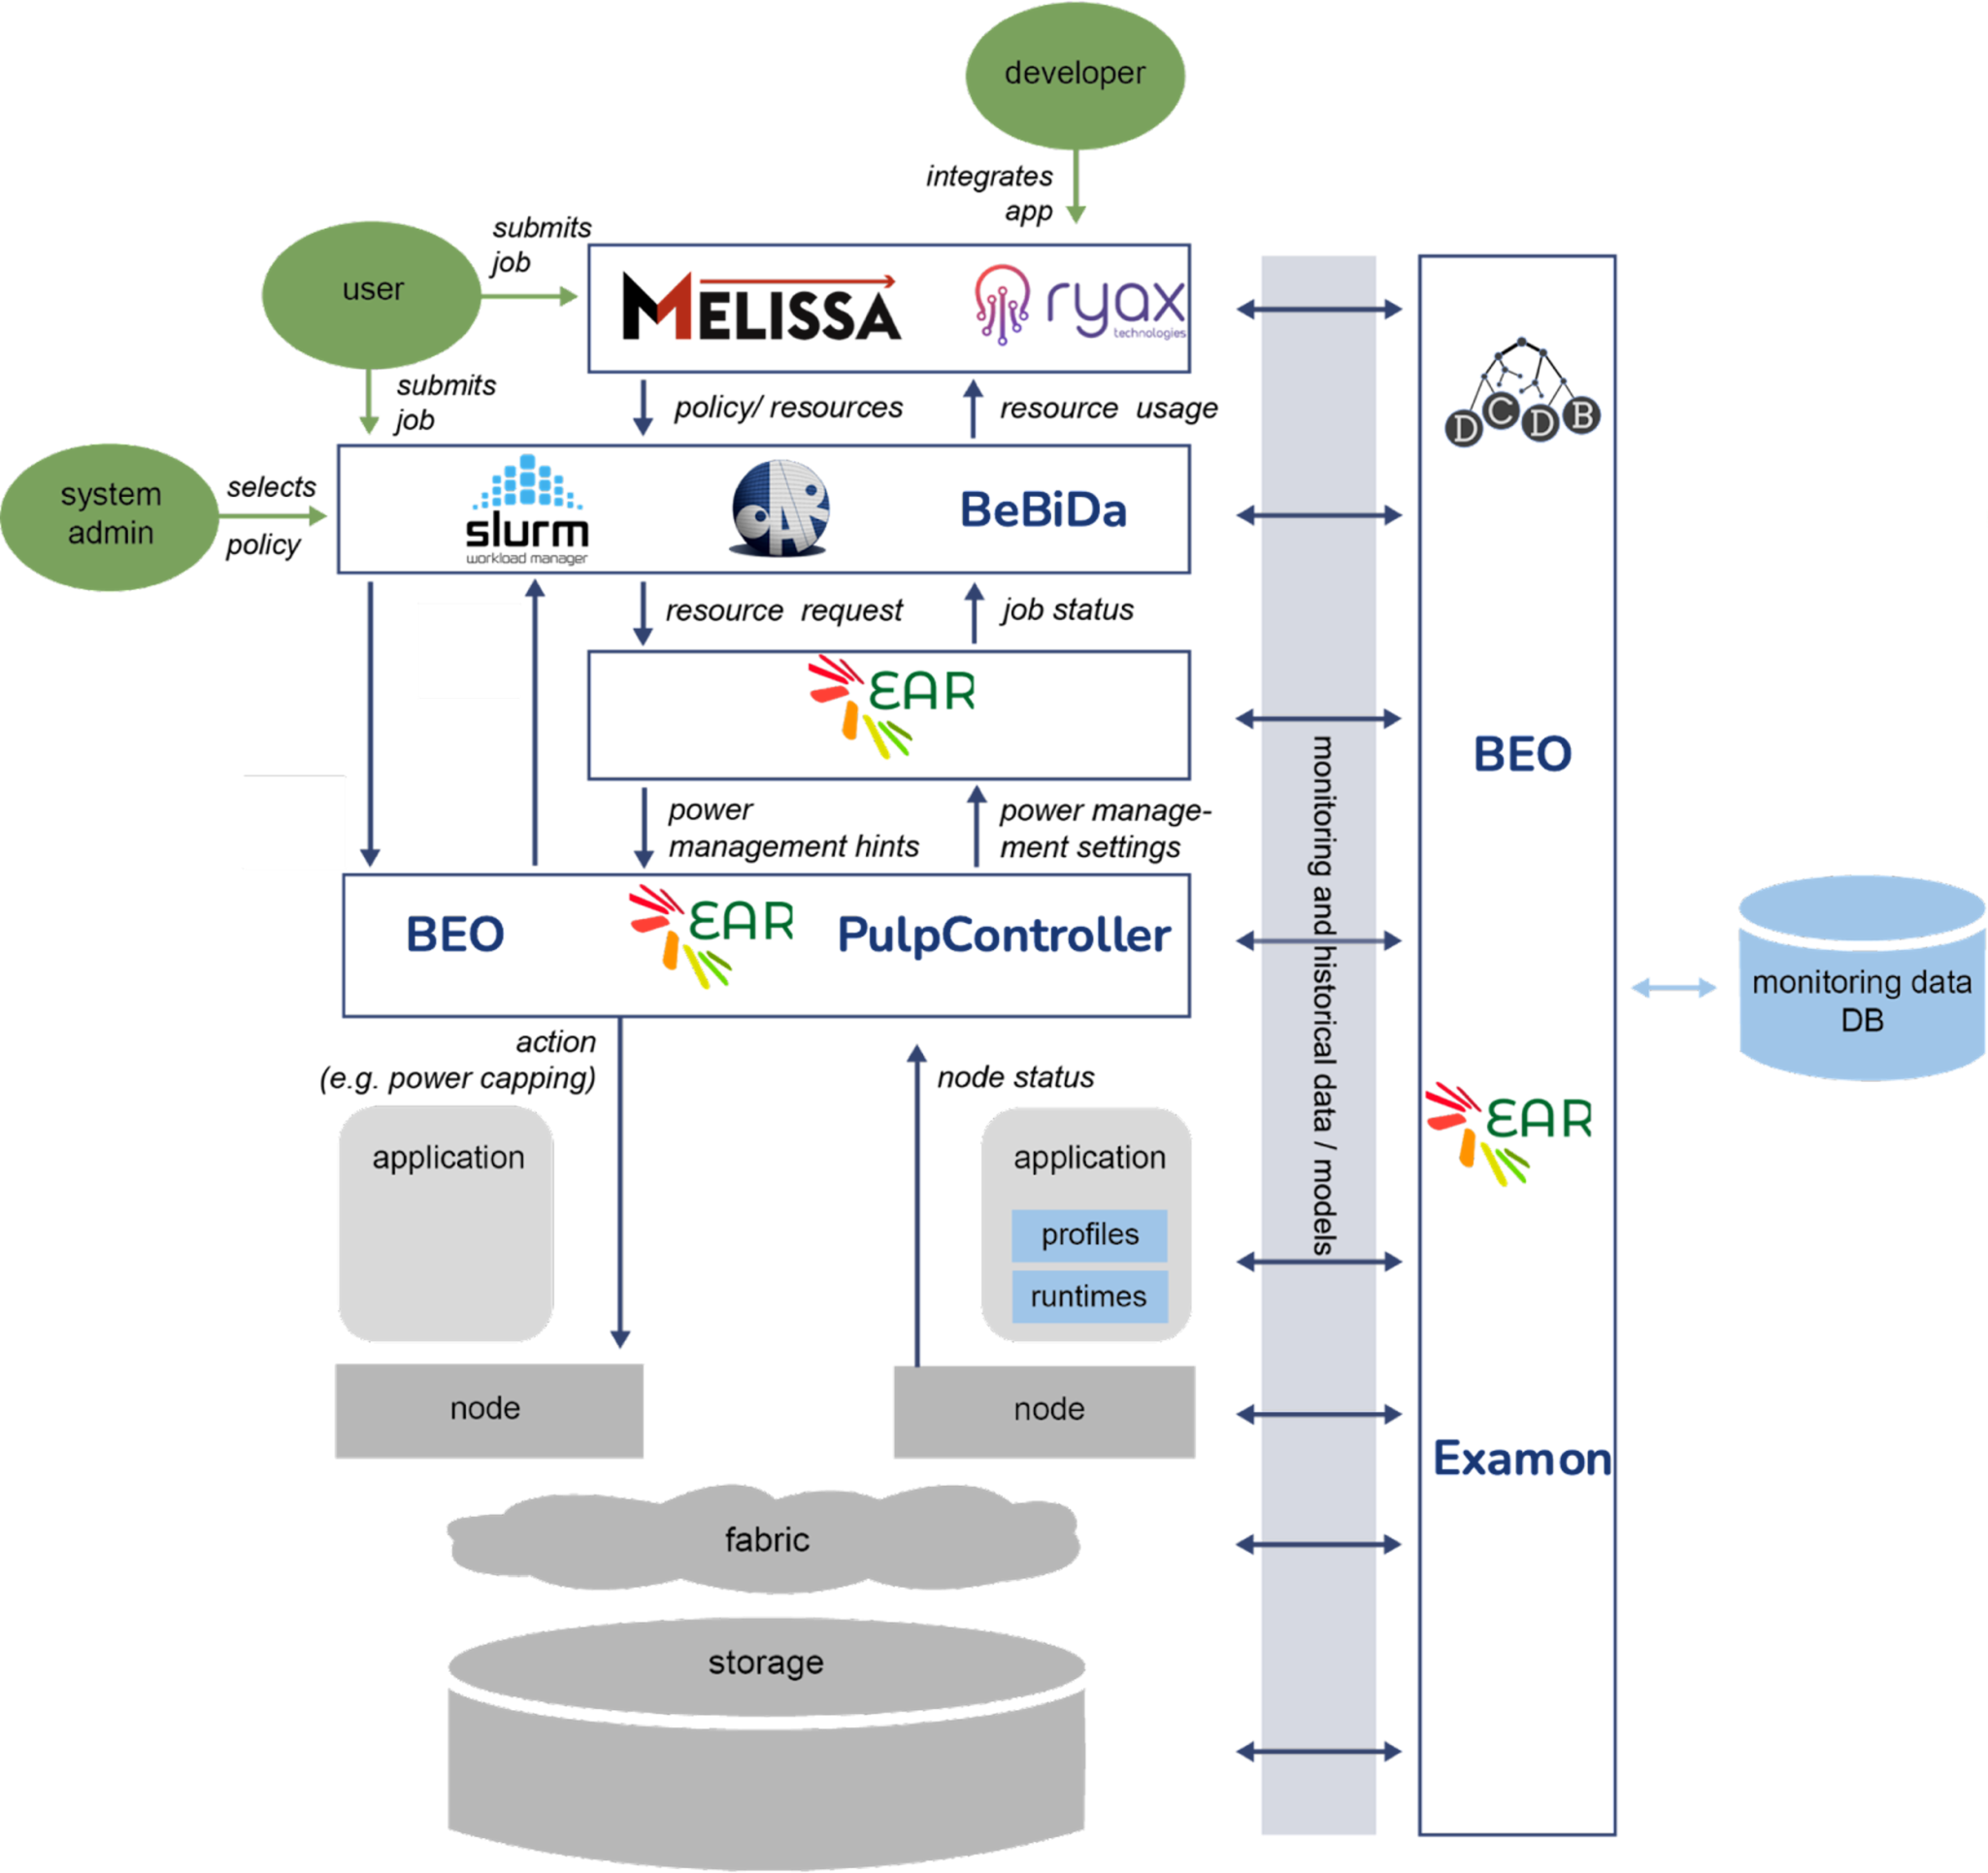
\includegraphics[width=\textwidth]{img/REGALE_USE.png}
    \caption{Copertura componenti}\label{fig:regale_cover}
    \end{subfigure}
    \caption{Implementazione dei componenti secondo il modello del Power stack}
\end{figure}

\section{Integrazione}
Vista la natura dei software introdotti nel progetto, non era previsto che questi potessero scambiare informazioni tra di loro, in quanto nati per essere usati singolarmente. Inoltre, data la difficoltà di creare interfacce di comunicazione, specifiche per ogni coppia di componente, si è scelto di procedere con un \textbf{middleware DDS} unificato. %Questa tesi è nata in collaborazione con REGALE, ed è stata stilata anche per riportare test utili alla finalità di REGALE.